\subsection{Machine Learning \--- Reformulation}

\subsubsection{Aim}

\begin{frame}
\frametitle{Aim}
Reformulation, what is it ?
%Asked questions are transformed in trees. But how to ensure the trees are adapted to our modules?
\pause


This is a translation module! % TODO too many exclamation points

\begin{exemple}
((United States,birth date,?),president,?) 

-> 

((United States,president,?),birth date,?)
\end{exemple}
%Changing the form, not the content.
\end{frame}

\subsubsection{Operation}
\begin{frame}
\frametitle{Operation}
Our tree is projected in a $\mathbb{R}$-vs: space of vectors.

\begin{defi}
The dictionary associates a vector triple to a vectors.
\end{defi}

\end{frame}

\begin{frame}
\frametitle{Projection}
\begin{tikzpicture}[x=2.5cm]
\node (s) at (1,0) {s};
\node (p) at (3,0) {p};
\node (r) at (2,1) {r};


\node (a) at (2,2) {a=compact(s,r,p)};
\node (b) at (4,2) {b};
\node (l) at (3,3) {l};
\node (h) at (3,4) {h=compact(a,l,b)};

\draw (s)--(a)--(p);
\draw (r)--(a);
\draw (a)--(h)--(b);
\draw (l)--(h);
\end{tikzpicture}
\end{frame}

\subsubsection{Build the request}

\begin{frame}
\frametitle{From vector to tree}

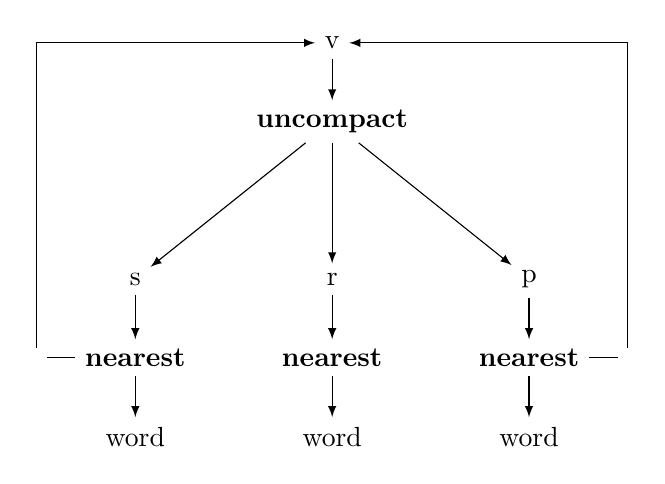
\begin{tikzpicture}[x=2.5cm]
\node (s) at (1,0) {s};
\node (p) at (3,0) {p};
\node (r) at (2,0) {r};
\node (sf) at (1,-1) {\textbf{nearest}};
\node (pf) at (3,-1) {\textbf{nearest}};
\node (rf) at (2,-1) {\textbf{nearest}};
\node (auxl) at (0.5,-1) {};
\node (auxr) at (3.5,-1) {};
\node (sw) at (1,-2) {word};
\node (pw) at (3,-2) {word};
\node (rw) at (2,-2) {word};
\node[rectangle] (b) at (2,2) {\textbf{uncompact}};
\node (a) at (2,3) {v};
%\node (b) at (4,2) {b};
%\node (l) at (3,3) {l};
%\node (h) at (3,4) {h=compact(a,l,b)};

\draw[->, >=latex] (b)--(s);
\draw[->, >=latex] (b)--(p);
\draw[->, >=latex] (b)--(r);
\draw[->, >=latex] (a)--(b);
\draw[->, >=latex] (r)--(rf);
\draw[->, >=latex] (p)--(pf);
\draw[->, >=latex] (s)--(sf);
\draw[->, >=latex] (rf)--(rw);
\draw[->, >=latex] (pf)--(pw);
\draw[->, >=latex] (sf)--(sw);

\draw[->, >=latex] (auxr)|-(a);
\draw[->, >=latex] (auxl)|-(a);
\draw (auxr)--(pf);
\draw (auxl)--(sf);
\end{tikzpicture}

\end{frame}

\subsubsection{Learn}

\begin{frame}
\frametitle{Training}
Semantic distance.

Use relation graph ``instance of'' from Wikidata.
\end{frame} 
